\documentclass[notes]{subfiles}
\begin{document}
	\chapter{Integration}
	\addcontentsline{toc}{section}{5.1 - Approximating Areas}
	\setcounter{section}{1}
	\fancyhead[RO,LE]{\bfseries \large \nameref{cs51}} 
	\fancyhead[LO,RE]{\bfseries \currentname}
	\fancyfoot[C]{{}}
	\fancyfoot[LO,RE]{\large \thepage}	%Footer on Right \thepage is pagenumber
	\fancyfoot[RO,LE]{\large Chapter 5.1}

\section*{Approximating Areas}\label{cs51}
	\subsection*{Before Class}
	\subsubsection*{Sigma Notation}
		\begin{rmk}[Sigma Notation]
			\emph{Sigma notation} is a shorthand way to write sums.  For example,
				\\ \\ \\ \\ \\
			Here,\blank{1} refers to the \emph{starting index}, and \blank{1} is called the \emph{ending index}.  
		\end{rmk}
		
		\begin{ex}
			Write the following using sigma notation:
			\begin{enumerate}[(a)]
				\item \(1 + 2 + ... + 20\)
					\vs{1}
					
				\item \(2 + 4 + ... + 50\)
					\vs{1}
					
				\item \(1 + \dfrac{1}{2} + \dfrac{1}{4} + \dfrac{1}{8} + \dfrac{1}{16} + \dfrac{1}{32}\)
					\vs{1}
			\end{enumerate}
		\end{ex}
			\newpage
			
		\begin{center}
				\tabulinesep = 4mm
				{\setlength{\arrayrulewidth}{1.5pt}
				\begin{tabu}{| X[l] X[l] | X[l] X[l] |}\hline
					\multicolumn{2}{|c|}{\large{\textbf{Helpful Formulas}}} & \multicolumn{2}{c|}{\large{\textbf{Rules for Sigma Notation}}} \\
					 $\ds \sum_{i=1}^n i$ & $ \dfrac{n(n+1)}{2}$	& $\ds \sum_{i=1}^n c  $	& $nc$ \\ 
					 $\ds \sum_{i=1}^n i^2$ & $\dfrac{n(n+1)(2n+1)}{6}$	& $\ds \sum_{i=1}^n ca_i$	& $c\ds\sum_{i=1}^n a_i$ \\
					 $\ds \sum_{i=1}^n i^3$ & $\lrpar{\dfrac{n(n+1)}{2}}^2$	& $\ds \sum_{i=1}^n (a_i\pm b_i)$ & $\ds\sum_{i=1}^n a_i \pm \sum_{i=1}^n b_i$ \\ \hline
				\end{tabu}
				}
			\end{center}
			
		\begin{ex}
			Evaluate the following:
			\begin{enumerate}[(a)]
				\item \(\ds \sum_{i=1}^{100} (i-1)^2\)
					\vs{1}
					
				\item \(\ds \sum_{i=1}^6 (i^3 - 2i^2)\)
					\vs{1}
					
				\item \(\ds \sum_{k=1}^{15} (3k - 2)\)
					\vs{1}
			\end{enumerate}
		\end{ex}
			\newpage
			
	\subsubsection*{Approximating Area}
		\begin{ex}
			  The function \(y = x^2\) on the interval \([0,1]\) is graphed below.
			\begin{center}
				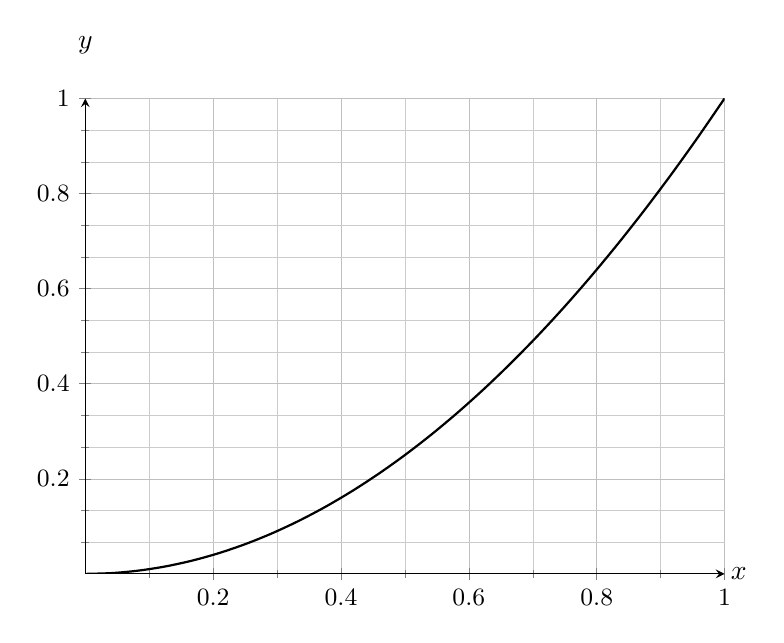
\begin{tikzpicture}
					\begin{axis}[
						height = 3in,
						width = .8\textwidth,
						grid = both,
						grid style={line width=.1pt, draw=gray!10},
						major grid style={line width=.2pt,draw=gray!50},
						minor grid style={line width=.2pt, draw=gray!40},
						every tick label/.append style={font=\small},
						axis x line = middle,
						axis y line = middle,
			    			every axis y label/.style={at={(ticklabel cs:1.15)}},
			    			%ytick = {-4, -2, -3, -1, 1, 2, 3, 4},
						y label style={at={(axis description cs:0,1.15)},anchor=north},
			    			ylabel = {$y$},
		    				every axis x label/.style= {at ={(ticklabel cs:1)}},
		    				%xtick = {-4,-3,-2,-1,1,2,3,4},
		    				x label style={at={(axis description cs:1.05,.0)},anchor=east},
		    				xlabel = {$x$},
		    				xmin = 0, xmax = 1,
		    				minor y tick num = 2,
		    				minor x tick num = 1
					]
					
						\addplot[thick, smooth, domain = 0:1] {x^2};
					\end{axis}
				\end{tikzpicture}
			\end{center}
		\begin{enumerate}[(a)]
			\item Use four rectangles to approximate the area under the parabola \(y = x^2\) from 0 to 1; start from the left endpoint, 0.
				\vs{1}
				
			\item There are two ways of drawing the four rectangles; approximate the same area by starting with the right endpoint, 1.
				\vs{1}
		\end{enumerate}	
		\end{ex}	
			\newpage
			
		\begin{ex}
			Use eight rectangles to approximate the area under \(y = x^2\) from 0 to 1, using both left and right endpoints.  Compare your estimates to the previous two calculations.
			\begin{flushleft}
				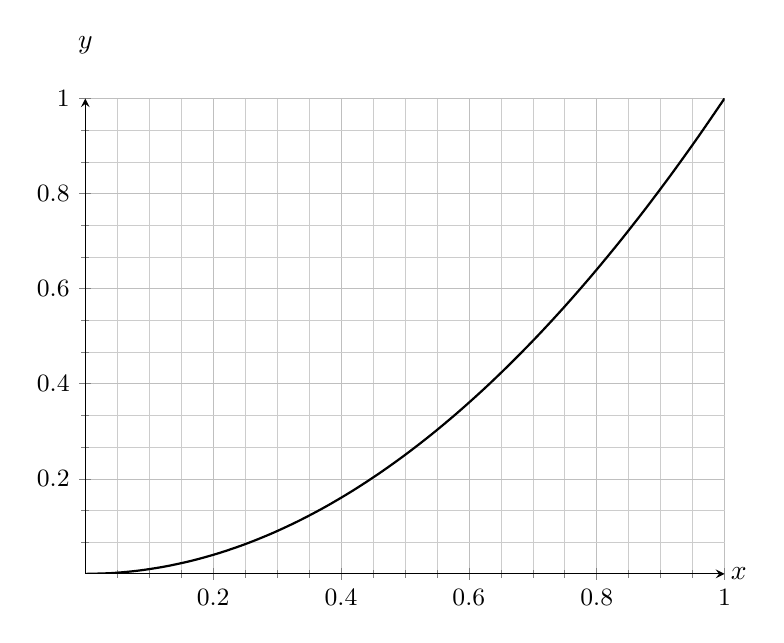
\begin{tikzpicture}
					\begin{axis}[
						height = 3in,
						width = .8\textwidth,
						every tick label/.append style={font=\small},
						axis x line = middle,
						axis y line = middle,
						grid = both,
						grid style={line width=.1pt, draw=gray!10},
						major grid style={line width=.2pt,draw=gray!50},
						minor grid style={line width=.2pt, draw=gray!40},
			    			every axis y label/.style={at={(ticklabel cs:1.15)}},
			    			%ytick = {-4, -2, -3, -1, 1, 2, 3, 4},
						y label style={at={(axis description cs:0,1.15)},anchor=north},
			    			ylabel = {$y$},
		    				every axis x label/.style= {at ={(ticklabel cs:1)}},
		    				%xtick = {-4,-3,-2,-1,1,2,3,4},
		    				x label style={at={(axis description cs:1.05,.0)},anchor=east},
		    				xlabel = {$x$},
		    				xmin = 0, xmax = 1,
		    				minor y tick num = 2,
		    				minor x tick num = 3
					]
					
						\addplot[thick, smooth, domain = 0:1] {x^2};
					\end{axis}
				\end{tikzpicture}
			\end{flushleft}
		\end{ex}
			\vs{3}
			
		\begin{question}
			What do you think would happen to our approximation of area if we used more\\[5pt] rectangles?
		\end{question}
			\vs{.5}
			\newpage
	
	\subsection*{Pre Class Practice}
		
		\begin{ex}
			Suppose that \(\ds \sum_{i=1}^{100}a_i = 15\) and \(\ds \sum_{i=1}^{100}b_i = -12\). Determine the value of the following:
			\begin{enumerate}[(a)]
				\item \(\ds \sum_{i=1}^{100} (a_i + b_i)\)
					\vs{1}
					
				\item \(\ds \sum_{i=1}^{100} (a_i - b_i)\)
					\vs{1}
					
				\(\ds \sum_{i=1}^{100} (2a_i  -3b_i)\)
					\vs{1}
			\end{enumerate}
		\end{ex}
		
		\begin{ex}
			Use 4 right rectangles to approximate the area under the curve \(\cos (\pi x)\) on the inteval \([0,1]\)
		\end{ex}
			\vs{2}
			
		\newpage
		
	\subsection*{In Class}
	\subsubsection*{Estimating Area}
		Generically, the process we are following has the following steps:
		\begin{rmk}[Approximating Area Under a Curve]
			\begin{enumerate}[(1)]
			\setlength\itemsep{30pt}
				\item 
				\item 
				\item 
				\item 
			\end{enumerate}
		\end{rmk}
		
		\begin{question}$ $
			\begin{enumerate}[(a)]
				\item If the interval we are concerned about is \([a,b]\), and we are using \(n\) rectangles to approximate the area, how could we write the base length of each individual rectangle?  Denote the length by \(\Delta x\).
					\vs{1}
					
				\item Let \(a = x_0\).  How could we express \(x_1\)?  \(x_2\)?  What about a generic \(x_i\), where \(1\leq i\leq n\)?
					\vs{1}
					
				\item Let \(f(x_i)\) be the function value at \(x_i\).  Using (a) and (b), write an expression for \(S_n\), the sum of areas of our approximating rectangles.
					\vs{1}
			\end{enumerate}
		\end{question}
			\newpage
			
		\begin{defn}[Area Under a Curve]
			The \textbf{area} of the region $S$ that lies under the graph of the continuous function $f$ is the limit of the sum of the areas of approximating rectangles:\\
					\vspace{.5in}
				
				or
				
					\vspace{.5in}		
		\end{defn}
			
		\begin{rmk}[Left Rectangle Approximation]
			The left rectangle approximation for the area under the curve $f(x)$ on the interval $[a,b]$ (using $n$ rectangles) is given by
				\vspace{.75in} \\
			
			or, in sigma notation,
				\\ \\ \\ \\
			
			The \(n\)th left rectangle approximation is denoted \(L_n\).
		\end{rmk}
			\vs{.25}

		\begin{rmk}[Right Rectangle Approximation]
			The right rectangle approximation for the area under the curve \(f(x)\) on the interval \([a,b]\) (using \(n\) rectangles) is given by\\[50pt]
			
				\vspace{.5in} \\
			
			or, in sigma notation,
			
				\\ \\ \\ \\
			
			The \(n\)th right rectangle approximation is denoted \(R_n\).
		\end{rmk}
			\vs{.25}
			\newpage
			
		\begin{ex}
			Consider \(f(x) = \dfrac{1}{x}\).
			\begin{enumerate}[(a)]
				\item Carefully sketch the graph of \(f(x)\) on the interval \([1,4]\).
					\vs{2.5}
					
				\item Find \(R_3\), and draw the rectangles on your sketch.
					\vs{1}

				\item Express the sum from (b) in sigma notation.
					\vs{.5}
					
				\item Find \(L_3\), and draw the rectangles on your sketch.
					\vs{1}
					
				\item Express the sum from (d) in sigma notation.
					\vs{.5}
					
			\end{enumerate}
		\end{ex}
			\newpage
			
		\begin{ex}
			Again, consider \(f(x) = \dfrac{1}{x}\) on \([1,4]\).
			\begin{enumerate}[(a)]
				\item Resketch the graph of \(f(x)\).
					\vs{1}
					
				\item Find \(R_6\), and include the rectangles on your sketch from (a).  How do these rectangles compare to the \(R_3\) rectangles?
					\vs{1}
					
				\item Find \(L_6\), and include the rectangles on your sketch from (a).  How do these rectangles compare to the \(L_3\) rectangles?
					\vs{1}
 
			\end{enumerate}
		\end{ex}
			\newpage
			
	
		\begin{ex}
			For \(f(x) = 5-x^2\), identify the upper/lower (aka right/left) sums for \(n = 5\).
		\end{ex}
			\vs{1}
			
		\begin{ex}
			Approximate the area under \(f(x) = \cos x\) between \(x=0\) and \(x = \dfrac{\pi}{4}\), using \(n = 4\).
		\end{ex}	
			\vs{1}
			\newpage
			
		\begin{ex}
			For \(f(x) = x^2\) on \([0,1]\), show that the sum of the areas of the upper approximating rectangles approaches \(\dfrac{1}{3}\), i.e. \(\ds \lim_{n\to\infty} R_n = \dfrac{1}{3}\).
		\end{ex}
			\vs{1}
			\newpage
			
	\subsection*{After Class Practice}
		\begin{ex}
			Find \(R_6\) and \(L_6\) for \(f(x) = \dfrac{1}{x^2+1}\) on the interval \([-1,5]\)
		\end{ex}
			\vs{3}
			
		\begin{ex}
			Let \(r_j\) denote the total rainfall in Portland on the \(j\)th day of the year 2009. Write a sentence interpreting the sum \(\ds \sum_{j=1}^{31} r_j\).
		\end{ex}
			\vs{1}
\clearpage
\end{document}